
\chapter {Haptics rendering algorithms}
\label{secHapticsRenderingAlgorithms}
In HAPI a haptics rendering algorithm (or haptics renderer) is a class
responsible for determining the forces and torque to render depending
on position and other data from the haptics device and all the shapes
the user has added to the scene. 

\section{Proxy based rendering}
All the algorithms supported by HAPI (both internally implemented and
external libraries such as OpenHaptics and Chai3D) use some variant of
proxy based haptics rendering. The proxy based rendering technique
involves having a virtual representation of the haptics device called
the proxy. The proxy follows the position of the haptics device, but
is not allowed to penetrate any surface. This means that when a
shape is touched the proxy stays on the surface of the object, even
if the haptics device actually has penetrated the surface. Forces are
then generated to bring the haptics device out of the surface, towards
the proxy, and usally some kind of spring force between the proxy and
haptics device is used ( see figure \ref{Proxy-probe} ). When the user 
moves the haptics device inside
the object the proxy follows the movement, but on the surface. How the
proxy follows determines how the structure of the surface will
feel. For example, if the proxy is always moved to a local minimum on
the distance to the surface, the surface will feel completely smooth,
but if the proxy is dragging behind friction effects are felt. In
HAPI the user can control both the forces generated and the movement
of the proxy.

\begin{figure} 
  \centering 
  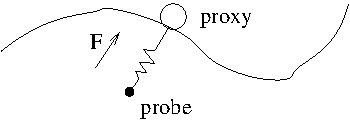
\includegraphics{images/proxyfinger.pdf}
  \caption{The proxy stays on the surface when the haptics
  device (probe) penetrates the surface. The resulting force is most
  commonly a spring force pushing the probe back towards the proxy.} 
  \label{Proxy-probe} 
\end{figure}



In the algorithms in HAPI the shape of the proxy is either a point
or a sphere. The problem with point proxies is that it can fall
through small gaps in the haptic shape and makes it very hard to be able
to touch small, thin objects. The problems with spheres, as with
all other proxy-shapes than point, is that with
increasing complexity of the proxy the problem of constraining the
proxy to a surface increases. As the complexity increases the problem usually
require more calculations to solve and as such it can be hard to
make an algorithm fast enough for haptics rendering.

\section{Available renderers}
There are four haptic renderers available in HAPI, where two are internally
implemented in HAPI and two uses external haptics libraries. Each of them can work better than the others on a specific shape model or in a specific application. You will have to try and see which one works best in your case and with your requirements. In the listing below we point out some of the strength and weaknesses of each renderer in order for you to choose the algorithm. 

\subsection{GodObject renderer}
The god-object algorithm is based on the paper ``A constrained based god-object method for haptics display'' by Zilles et al. \cite{zilles95constraintbased}. It uses a point proxy and supports custom user defined surfaces.

\begin{minipage}[t]{3in}
\subsubsection{Pros} 
\begin{itemize} 
\item Open source. 
\item Device independent. 
\item User surfaces. 
\end{itemize} 
\end{minipage}
\begin{minipage}[t]{3in}
\subsubsection{Cons} 
\begin{itemize} 
\item Could be problems with the concave part of a curved surface.
\end{itemize}
\end{minipage}


\subsection{Ruspini renderer}
The RuspiniRenderer is based on the algorithm presented by Ruspini in
``The Haptic Display of Complex Graphical Environments'' \cite{ruspini}.
It is different from all the other renderers in HAPI in that it uses a
sphere proxy making it possible to have an interaction object with a size instead of just a point.  

\begin{minipage}[t]{3in}
\subsubsection{Pros}
\begin{itemize}
\item Open source.
\item Device independent.
\item User surfaces.
\item Sphere proxy.
\end{itemize}
\end{minipage}
\begin{minipage}[t]{3in}
\subsubsection{Cons}
\begin{itemize}
\item A little slower than other renderers in HAPI.
\end{itemize}
\end{minipage}

\subsection{Chai3D}
Chai3D \cite{chai3d} is an open source haptics library distributed under the GNU GPL license. It has been developed by a team at Stanford University in California, USA. 

\begin{minipage}[t]{3in}
\subsubsection{Pros}
\begin{itemize}
\item Open source.
\item Device independent.
\end{itemize}
\end{minipage}
\begin{minipage}[t]{3in}
\subsubsection{Cons}
\begin{itemize}
\item No user defined surfaces.
\item Some fallthrough problems on moving objects.
\end{itemize}
\end{minipage}

\subsection{OpenHaptics}
OpenHaptics \cite{openhaptics} is a proprietary haptics library developed by SensAble Technologies. It uses a point proxy based approach and provides a stable haptic feedback. It is however not very extendable in terms of user defined surfaces and only works with haptics from SensAble Technologies.

\begin{minipage}[t]{3in}
\subsubsection{Pros}
\begin{itemize}
\item MagneticSurface available.
\item Good with moving objects.
\end{itemize}
\end{minipage}
\begin{minipage}[t]{3in}
\subsubsection{Cons}
\begin{itemize}
\item Only works with devices from SensAble.
\item No user defined surfaces.
\item Closed source.
\end{itemize}
\end{minipage}


\section{Surfaces}
A surface object in HAPI is an object that defines the haptic properties of a geometric shape, such as stiffness and friction. It is responsible for generating forces at a local contact point on a shape. The base class of all such objects is HAPISurfaceObject and there are several surfaces available in HAPI. 

\begin{itemize}
\item FrictionSurface - Allows the user to set stiffness, damping, static friction and dynamic friction parameters. The force produced is a linear spring-damper force between the proxy position and probe position, i.e. F = stiffness * (proxy\_pos - probe\_pos) - damping * probe\_velocity. The friction parameters control how the proxy move over the surface during contact. The static friction parameter controls how hard it is to start moving across the surface from a resting contact while the dynamic friction parameter controls how hard it is to move across the surface when the proxy has started moving.
\item DepthMapSurface - Use a texture to define the depth of the surface (only available for GodObjectRenderer and RuspiniRenderer). A minimization algorithm controls how the proxy move over the surface. If the proxy is in an area on the surface that is considered deep it will be harder to move the proxy to an area on the surface which is considered higher. The depth calculated also modifies the force so that deep (and high) parts of the surface can be felt.
\item HapticTexturesSurface - A surface similar to FrictionSurface with the exception that the four parameters stiffness, damping, static\_friction and dynamic\_friction are modified by textures given to the surface.
\end{itemize}

There is also a surface specific for the OpenHaptics
library which allows the user to set the parameters available in
that library directly. That surface is:
\begin{itemize}
\item OpenHapticsSurface - Has all the parameters available in
  OpenHaptics, i.e. stiffness, staticFriction, etc, but instead of
  specifying them in the HAPI way in absolute units, they are all
  specified as a value between 0 and 1. A value of 0 for the stiffness
  means no stiffness at all and a value of 1 means the maximum
  stiffness the device can handle. See doxygen documentation for all
  parameters of this surface.
\end{itemize}

\subsection{User defined surfaces}
In addition to using the already defined surfaces HAPI provides an interface to develop custom surfaces.
This gives the user full control over the forces generated when in contact with a surface.
The base class for all surface classes is HAPISurfaceObject. The surface object is responsible for two things. 


\subsubsection{Moving the proxy}
The movement of the proxy is often used to control the feeling of an object when moving across the surface, e.g. if the surface should feel smooth or rough. Letting the proxy move along the contact plane as to minimise the distance between proxy and probe will create a totally smooth surface since the forces will always just be normal forces and no tangential forces ( see figure \ref{proxy movement} ). Letting the proxy lag behind in different ways can be used to create different friction-like effects and not letting it move at all forces the proxy to be stuck at the first point of contact of the surface (unless the probe is lifted out of the surface). The proxy movement is a 2D movement along the xz-plane of the local contact coordinate system. 

When defining a new surface the virtual function getProxyMovement( ContactInfo \&ci ) in HAPISurfaceObject is used to define the proxy movement. The user should call the ci.setLocalProxyMovement( Vec2f \&pm ) function here to set the proxy movement. The rendering system will try to move the proxy according to the specified movement but might be stopped by colliding with other shapes along the path to the new position. The proxy will then stay at this collision point instead of moving all the way to the specified position.

\begin{figure} 
  \centering 
  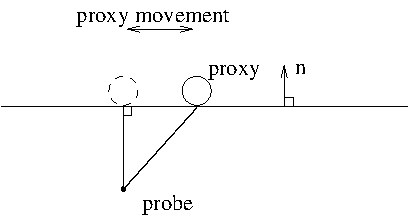
\includegraphics{images/surface.pdf}
  \caption{Local surface contact. Always moving the proxy to the dashed position(i.e. minimise the distance between proxy and probe) will give a surface without any friction.}
  \label{proxy movement} 
\end{figure}

\subsubsection{Calculating an interaction force}
After the new position of the proxy has been calculated, the interaction force with the surface has to be determined. For the most common surface types this is usually a linear spring force pulling the device back towards the proxy. It is however totally up to the user to define the force profile of the interaction to model e.g. button clicks and other non-linear behaviour. To have the most stable force feedback it is recommended that the direction of the force is towards the proxy.  
The interaction force(and possible torque) in a new surface is determined by defining the virtual function getForces( ContactInfo \&ci ) by calling the setGlobalForce or setLocalForce functions in the ci object. 

\subsection{The ContactInfo object}
When calculating the proxy movement and the interaction force the user has access to a ContactInfo object. This object contains information about the surface contact that can be used in the calculations. It is also the object in which to return the calculated forces and proxy movement. The most commonly used values provided are:

\begin{itemize}
\item Contact point origin.
\item Probe position.
\item Probe velocity.
\item Texture coordinate of contact.
\item The haptics device that made the contact.
\item The haptic shape the contact is made on.
\end{itemize}


All positions can be obtained in either the global coordinate system or
in a local contact coordinate system. The local coordinate system is constructed with the proxy position as the origin, the contact normal as the y-axis and and two arbitrary perpendicular axis in the plane as x and z-axis ( see figure \ref{coordsystems} ). This means that e.g. the penetration depth is the same as -y in the local coordinate system. There are also functions in the ContactInfo object for converting between these two coordinate spaces. 

\begin{figure} 
  \centering 
  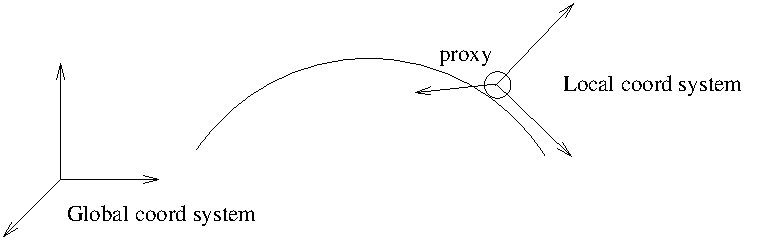
\includegraphics{images/coordsystems.pdf}
  \caption{Local and global coordinate system. The local coordinate system is constructed with the proxy position as the origin, the contact normal as the y-axis and and two arbitrary perpendicular axis in the plane as x and z-axis.}
  \label{coordsystems} 
\end{figure}

The output parameters that can be set are:

\begin{itemize}
\item Force - setGlobalForce/setLocalForce
\item Torque - setGlobalForce/setLocalForce
\item Proxy movement - setLocalProxyMovement
\end{itemize}

See the Doxygen documentation for a full listing of the functions available.

\subsection{Example surface}
Following is an example of an implementation of a surface with no friction and a linear spring force for the penetration of the surface.   

\input{examples/surface_example_h}

